% Due

\documentclass[a4paper]{article}

\usepackage[english]{babel}
\usepackage[utf8]{inputenc}
\usepackage{amsmath}
\usepackage{graphicx}
\usepackage{parskip}
\usepackage{amssymb}
\usepackage{mathtools}
\usepackage{upgreek}
\usepackage{svg}
\usepackage{todonotes}

\DeclarePairedDelimiter\ceil{\lceil}{\rceil}
\DeclarePairedDelimiter\floor{\lfloor}{\rfloor}

\title{ECE358 Assignment 7}
\author{Ariel Weingarten --- 20366892\\
        Alexander Maguire --- }
\date{\today}

\begin{document}

\maketitle

%(10 points) Let G be a weighted undirected graph that represents a network.
% (a) Give an example of G and events as discussed below, that demonstrate the following behaviour. Assume that poisoned reverse is in effect. Initially, running a Distance-Vector routing protocol on G results in no routing loops. After we converge, events occur that cause the routing protocol to be run again among some nodes of G, and we end up with a routing loop that comprises 4 nodes. (i.e., for some destination, A forwards to B, which forwards to C, which forwards to D, which in turn forwards to A.)
% (b) In what way would using path vector routing address the above behaviour demonstrated by G? (In path vector routing, not only distance vectors are sent between routers, but also the paths that correspond to those distances.)
\section{Question 1}
\subsection{Part One}
\begin{enumerate}
	\item \begin{enumerate}
		\item B's connection to E goes down\\
	\end{enumerate}

	\item \begin{enumerate}
		\item B responds by telling its neighbors that its (B's) new distance to E is infinity\\
		\item A wants to send a message to E and it sends that message to B. (because it is in the process of receiving the update from B)\\
		\item C's connection to E goes down\\
	\end{enumerate}

	\item \begin{enumerate}
		\item B forwards A's message to C\\
		\item C tells neighbours that its distance to E is infinity\\
	\end{enumerate}

	\item \begin{enumerate}
		\item C forwards A's message to D\\
		\item D forwards the message to A because it knows that C is infinity away and has not received any updates from A yet. The loop has been completed and whether or not it continues is a matter for another question.\\
	\end{enumerate}

\end{enumerate}

\subsection{Part Two}
In step 3b in the previous section C actually knows that there no longer exist any routes to E because it has received
the update from B in step 2a and it has just seen that it's own link has gone down. It may seem that C would try to
send the message to D, but from the problem statement we know that the path vector protocol has already been run and
C would know that D's route was through C and that there are no more options to deliver the message.


% (5 points) Let H: {0,1}∗ −→ {0,1}c, for some constant c, be a uniform random function. What is the number of evaluations of H(·) we expect to have to perform to find three inputs that collide?
\section{Question 2}
Let $X$ be a discrete random variable that represents the number of collisions from hashing input values. Let $Y_{ijk}$ be the discrete random variable that is 1 if inputs $i$, $j$, and $k$ collide or 0 if they do not. This represented by the following equation:
$$
X = \sum\limits_{i=1}^{n-2} \sum\limits_{j=2}^{n-1} \sum\limits_{k=3}^{n} Y_{ijk}
$$

To solve for the number of evaluations we can set X >= 1:

$$
1 \leq  \frac{1}{m^2}\cdot {n \choose{3}}
$$
Which can be written as:

$$
1 \leq \frac{n(n-1)(n-2)}{6m^2}
$$

$$
6m^2 \leq n(n-1)(n-2)
$$

This does not expand nicely, so I've asked my best bro Wolfram to help me out.

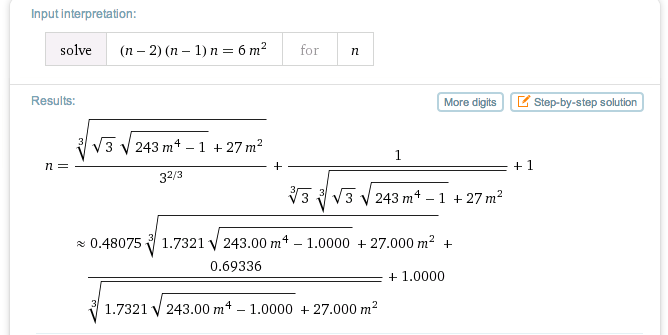
\includegraphics[width=1\textwidth]{a7q2.png}



% (5 points) Let the encryption scheme for a public-private key-pair <k, k−1> be: E(x) = {r}k || G(r) ⊕ x
% where r is a random number that is generated anew for each instance of encryption, G(·) is a random number generator that is a function of the input seed, and “||” is string-concatenation. Show that the scheme is not secure against a chosen ciphertext attack mounted by a polynomial-time adversary. (Hint: one way to fix the problem is to change the encryption operation to E(x) = {r}k || G(r) ⊕ x || H(r||x), where H is a hash function.)
\section{Question 3}
This scheme is not secure because it does not guarantee the integrity of the message.
If the attacker knows what x is or the structure of x, then they can modify the message to read whatever
they'd like and the receiver has no way to know that the message has been modified.
Adding the hash, $H(r||x)$ fixes this problem because the attacker can never know what $r$ is.
If the attack tries to modify the message in-flight, then the receiver will be able to check the message against the hash and discover the tampering.

% (5 points) Consider the zero-knowledge proof for quadratic-residuosity from my notes, which, in turn, is from Goldwasser et al. [GMR89]. It appears that the server should always choose b = 1 because that is the only option that forces Alice to respond with something that has to do with y. Show that if Alice knows that the server will always choose b = 1, then she can successfully participate in the protocol for any n even when she does not know w.
\section{Question 4}

%(5 points) From Section 4, Example 3.4 of Abadi and Needham [AN95]: “We leave the construction of an attack as an exercise for the reader.” Construct an attack. (You can use their proposed resolution as a hint.)
\section{Question 5}
Consider a malicious server Y that wants to make B think it is talking to A. If A
begins communication with Y, then here is an attack where Y obtains A's certificate and
uses it to fool B into thinking that it is communicating with A.

\begin{align*}
	A \longrightarrow Y &: \{K_{AY}\}_{K_{Y}}\\
	Y \longrightarrow B &: \{K_{AY}\}_{K_{B}}\\
	B \longrightarrow Y &: \{N_B\}_{K_{AY}}\\
	Y \longrightarrow A &: \{N_B\}_{K_{AY}}\\
	A \longrightarrow Y &: \{CA,\{N_b\}_{K_A^{-1}} \}_{K_{AY}}\\
	Y \longrightarrow B &: \{CA,\{N_b\}_{K_A^{-1}} \}_{K_{AY}}\\
\end{align*}

% (5 points) In Section 5, Example 5.2 of Abadi and Needham [AN95], fix the message so that B can be convinced that A knows X. Your solution should have all the security properties of the existing solution plus this.
\section{Question 6}
A can XOR $X$ with $H(X)$, making the message:
$$
A \longrightarrow B \text{:} \{X\}_B \{ H(X) \oplus X \}_{A^{-1}}
$$

% (5 points) In Section 6.2, Example 9.1 of Abadi and Needham [AN95], suppose that Message 5 is A −→
% B:{Nb}Kab (i.e.,withoutthe“+1”).Showanattackontheprotocol.
\section{Question 7}
A malicious third-party, C, could intercept message 4 and simply send it back to B. It would still face the difficulty of decrypting the messages that B sends it, but it can at least establish a session.

% (5 points) Suppose that a malicious principal E acquires Kab from a prior run of the Needham-Schroeder symmetric-key authentication protocol in Section 6.2, Example 9.1 of Abadi and Needham [AN95]. Show how E can compromise (or “deceive,” as the paper puts it) B as a consequence.
\section{Question 8}
E can obtain the nonce that B sends to A in Message 4. Then E can use $K_{ab}$ to decrypt the nonce, add one to it, then re-encrypt it with $K_{ab}$ to send back to B before A does in Message 5.


\end{document}
